\documentclass[11pt,a4paper]{article}
\usepackage[utf8]{inputenc}
\usepackage[T1]{fontenc}
\usepackage[spanish,es-nodecimaldot]{babel}
\usepackage{geometry}
\geometry{margin=2.5cm}
\usepackage{graphicx}
\usepackage{booktabs}
\usepackage{amsmath,amssymb}
\usepackage{hyperref}
\usepackage{float}
\usepackage{caption}
\usepackage{listings}
\usepackage{xcolor}
\usepackage{lmodern}

\hypersetup{colorlinks=true,linkcolor=blue,citecolor=blue,urlcolor=blue}

% Configuración formal de listados para la traza de ejecución
\definecolor{codebg}{RGB}{248, 249, 250}
\definecolor{bordercolor}{RGB}{220, 224, 230}
\lstset{
    backgroundcolor=\color{codebg},
    basicstyle=\ttfamily\scriptsize,
    breaklines=true,
    captionpos=b,
    frame=single,
    rulecolor=\color{bordercolor},
    tabsize=2,
    showstringspaces=false
}

\title{Optimización por Enjambre de Partículas (PSO) para el Problema del Viajante de Comercio y Comparativa ACO vs PSO\\ \large Informe Técnico Oficial: Representación por Claves Aleatorias, Escalamiento Multiescala y Evaluación Head-to-Head}
\author{
  Nicolas Jacobo Mondragón Rey \\
  Nicolas Emilio Morantes Puentes \\
  Santiago Jose Rodríguez Gutierrez \\[0.8em]
  Curso de Introducción a la Inteligencia Artificial 2026 \\
  \small Inteligencia de Enjambre y Metaheurísticas (Sesión 09)
}
\date{Septiembre 2026}

\begin{document}
\maketitle

\begin{abstract}
Se presenta la formulación, diseño computacional y análisis empírico del algoritmo de Optimización por Enjambre de Partículas (\emph{Particle Swarm Optimization}, PSO) aplicado al Problema del Viajante de Comercio (\emph{Traveling Salesperson Problem}, TSP) sobre instancias euclidianas uniformes de $N \in \{20, 2.000, 200.000\}$ ciudades. Dado que el PSO canónico opera sobre espacios \textbf{continuos} y el TSP es combinatorio, se adopta la codificación por \textit{random keys} ($tour = argsort(x)$, $x \in [0,1]^N$) con las ecuaciones estándar de velocidad de tres componentes (inercia, memoria personal y memoria social), inercia decreciente $w:0{.}90 \to 0{.}40$, cota de velocidad $v_{\max}=0{.}20$ y parada por $S$ iteraciones sin mejora. La escala masiva se aborda con descomposición jerárquica en grilla $15\times15$ paralelizada con OpenMP ($\approx$225 celdas de $\approx$900 ciudades). Con $S=N$ partículas en el régimen serie, la instancia de $200.000$ ciudades converge a un circuito hamiltoniano válido en $4{.}4\text{ s}$ con un pico de \textbf{$11{.}6\text{ MB}$} ($\approx 13.800\times$ menor a la matriz densa de $160\text{ GB}$). La calidad, sin embargo, revela el límite de la representación: el enjambre colapsa prematuramente sobre claves casi idénticas y el gap frente al estimador de Beardwood crece de +87\% ($N=20$) a +1970\% ($N=200.000$), demostrando cuantitativamente que un optimizador continuo mal adaptado no compite en un problema combinatorio.
En la segunda parte se confronta este PSO con nuestra implementación ACO bajo protocolo estricto (mismas instancias, mismo presupuesto, multi-semilla): el ACO vence en calidad en las tres escalas (exceso 24\%/0.2\%/0.1\% frente a 90\%/850\%/1294\%) a cambio de $2$--$5\times$ más tiempo, empatando en memoria ($<12\text{ MB}$).
\end{abstract}

\part{Informe PSO}% ==============================================================================

% ==============================================================================
\section{Definición del Problema y Complejidad Combinatoria}
% ==============================================================================
El Problema del Viajante de Comercio (TSP) consiste en determinar el ciclo hamiltoniano de coste euclidiano mínimo que visite un conjunto discreto de $N$ vértices exactamente una vez y retorne al nodo de origen:
\begin{equation}
    \min_{\pi \in \Pi} L(\pi) = \sum_{i=1}^{N-1} d\left(c_{\pi(i)}, c_{\pi(i+1)}\right) + d\left(c_{\pi(N)}, c_{\pi(1)}\right)
\end{equation}
donde $c_i = (x_i, y_i) \in [0, 1]^2$ y $d$ es la distancia euclidiana. En un grafo completo no dirigido, $|E| = N(N-1)/2$ y el número de tours distintos es $|\Pi| = (N-1)!/2$: para $N=20$ ya son $\approx 6\times10^{16}$ (fuerza bruta imposible) y para $N=2.000$ del orden de $10^{5735}$. La matriz densa de $N=200.000$ exigiría $160\text{ GB}$ en \texttt{float32}, de modo que solo son viables métodos con memoria subcuadrática.

% ==============================================================================
\section{Análisis Matemático del Consumo de Memoria}
% ==============================================================================
El enjambre almacena tres vectores reales por partícula (posición $X$, velocidad $V$ y mejor personal $P$), es decir $3\cdot S\cdot N$ flotantes:
\begin{equation}
    M_{\text{enjambre}} = 12\cdot S\cdot N\ \text{bytes (float32)}.
\end{equation}
Con $S=N=2.000$ el enjambre ocupa $48\text{ MB}$: es el único punto donde este PSO consume \textbf{más} memoria que el ACO disperso (feromona de $64\text{ KB}$). En el régimen jerárquico cada celda ($\approx$900 ciudades, $S=32$) demanda $\approx 350\text{ KB}$ por arreglo, con picos medidos de $11{.}6\text{ MB}$ totales. No se materializa jamás ninguna matriz $N\times N$: las distancias se evalúan al vuelo y la decodificación reutiliza un único buffer de índices $O(N)$.

% ==============================================================================
\section{Formulación del Enjambre de Partículas (PSO)}
% ==============================================================================
Cada partícula $i$ conserva posición $x_i$, velocidad $v_i$, mejor personal $p_i$ y el enjambre comparte el mejor global $g$. La actualización estándar es:
\begin{equation}
    v_i(t+1) = w\,v_i(t) + c_1r_1\odot[p_i - x_i(t)] + c_2r_2\odot[g - x_i(t)], \qquad x_i(t+1) = x_i(t) + v_i(t+1),
\end{equation}
con $r_1, r_2 \sim U[0,1)$ por partícula. Los tres sumandos son inercia (continuidad), componente cognitiva (memoria individual) y componente social (memoria colectiva). Se aplica recorte $x \in [0,1]$ y cota $|v| \le v_{\max}$, y la inercia decrece linealmente $w:0{.}90\to0{.}40$ para explorar al inicio y estabilizar al final. Parámetros: $c_1=1{.}4$, $c_2=1{.}6$ (ejemplo calculado de la guía), $v_{\max}=0{.}20$, $p_i$ y $g$ por minimización, parada por máximo de iteraciones o $S$ iteraciones sin mejora.

% ==============================================================================
\section{Adaptación al TSP: Claves Aleatorias}
% ==============================================================================
La posición continua se decodifica por ordenamiento: $tour = argsort(x)$, con costo $O(N\log N)$ por evaluación más $O(N)$ de la longitud. La velocidad inicia en cero y la primera posición se copia como mejor personal. Esta codificación es el talón de Aquiles del método: mover las \textit{claves} hacia las claves de $g$ \textbf{no} acerca el \textit{tour} al tour de $g$, pues infinitos vectores codifican la misma permutación y vecinos en $[0,1]^N$ decodifican a tours arbitrariamente lejanos. El enjambre, por tanto, colapsa sobre una región de claves y el orden deja de correlacionarse con la geografía: estancamiento local sin convergencia al óptimo.

% ==============================================================================
\section{Metodología Experimental y Regímenes de Escala}
% ==============================================================================
\begin{center}
\begin{tabular}{@{}crrrc@{}}
\toprule Régimen & $N$ & $S$ (partículas) & $T$ (iters) & Parada $S$ \\
\midrule Serie & 20 & 30 & 300 & 50 \\
Serie + 2-opt & 2.000 & $N$ & 100 & 15 \\
Jerárquico ($15\times15$) & 200.000 & 32/celda & 40 & --- \\
\bottomrule
\end{tabular}
\end{center}
$S=N$ guarda simetría con el ACO ($m=n$). Las instancias son idénticas a las del ACO (mismo generador y semilla; verificado por \texttt{diff}), de modo que los tours son directamente comparables. Las celdas usan semilla propia (determinismo bajo OpenMP) y se cosen por vecino más cercano sobre centroides.

% ==============================================================================
\section{Resultados Experimentales y Discusión Técnica}
% ==============================================================================

\subsection{Traza de Ejecución y Validación de la Salida (\texttt{./bin/pso})}
\begin{lstlisting}
./bin/pso -n 20
Params: S=30 part. T=300 w=[0.90,0.40] c1=1.40 c2=1.60 vmax=0.20 S_stop=50
Densa teorica: 0.000 GB | enjambre: 0.01 MB
  it   1/300  mejor-global=8.12  mejor-it=8.12  w=0.900
  it   2/300  mejor-global=7.40  mejor-it=7.40  w=0.898
  it   3/300  mejor-global=6.52  mejor-it=6.52  w=0.897
  ...
  parada temprana en it 134 (S=50 sin mejora)
Evaluaciones totales = 9000 (S x T)
Referencia NN greedy: 4.33
Tour valido: SI | longitud = 5.95
Tiempos: PSO/jer=0.003s 2opt=0.000s TOTAL=0.003s
Memoria: RSS actual 3708 -> 3780 KB (+0.1 MB) | peak VmHWM 3708 -> 3780 KB

./bin/pso -n 2000   (extracto)
Params: S=2000 part. T=100 w=[0.90,0.40] c1=1.40 c2=1.60 vmax=0.20 S_stop=15
  it   2/100  mejor-global=1009.93  mejor-it=1019.13  w=0.895
  it   3/100  mejor-global=1009.93  mejor-it=1012.65  w=0.890
  it   4/100  mejor-global=1009.93  mejor-it=1016.49  w=0.885
  parada temprana en it 15 (S=15 sin mejora)
Tour valido: SI | longitud = 383.54   (el 2-opt rescata de ~1010 a 383)
Tiempos: PSO/jer=5.587s 2opt=0.001s TOTAL=5.599s
Memoria: RSS actual 3764 -> 3892 KB (+0.1 MB) | peak VmHWM 3764 -> 50644 KB

./bin/pso -n 200000   (extracto)
Params: S=32 part. T=40 w=[0.90,0.40] c1=1.40 c2=1.60 vmax=0.20 S_stop=0
Grilla 15x15 -> 225 celdas
Evaluaciones totales = 288000 (n_celdas x S x T)
Tour valido: SI | longitud = 6591.53
Tiempos: PSO/jer=4.533s 2opt=0.000s TOTAL=4.545s
Memoria: RSS actual 3728 -> 9716 KB (+6.0 MB) | peak VmHWM 3728 -> 11316 KB
\end{lstlisting}

\subsubsection{Análisis de Métricas de la Salida}
\begin{itemize}
    \item \textbf{Instancia $N=20$:} el récord desciende por escalones ($8{.}12 \to 7{.}40 \to 6{.}52 \to 5{.}95$) con $w$ decayendo visiblemente ($0{.}900 \to 0{.}678$); cada escalón es un tour estrictamente mejor. La parada $S=50$ corta en la iteración 134 de 300 (55\% de cómputo ahorrado). El resultado (5.95) queda \textbf{peor} que el voraz NN (4.33): el enjambre no supera ni a la heurística más simple.
    \item \textbf{Instancia $N=2.000$:} con $S=N=2.000$ partículas, el mejor de la inicialización ($\approx$1010, un tour casi aleatorio) \textbf{jamás mejora} en 14 iteraciones y la parada $S=15$ dispara en el primer instante posible. Todo el mérito (1010 $\to$ 383) corresponde al pulido 2-opt final de $0{.}001\text{ s}$: el PSO propone y el 2-opt dispone. El pico de $50{.}6\text{ MB}$ es el enjambre $2000\times2000\times3$ flotantes previsto en la Sección~2.
    \item \textbf{Instancia $N=200.000$:} $288.000$ evaluaciones sobre 225 celdas en $4{.}5\text{ s}$ con pico de $11{.}3\text{ MB}$: el andamiaje jerárquico funciona (rápido y liviano), pero cada mini-enjambre ($32\times40$) apenas supera un tour aleatorio por celda y la costura acumula el daño ($L=6591{.}53$).
\end{itemize}

\subsection{Escalabilidad Computacional y Barrido Multiescala}
\begin{center}
\begin{tabular}{@{}crrrrr@{}}
\toprule $N$ & evaluaciones & tiempo & pico & $L$ & gap BHH \\
\midrule 20 & 9.000 & 0.003\,s & 3.8\,MB & 5.95 & +87\% \\
100 & 9.000 & 0.03\,s & 3.8\,MB & 40.9 & +474\% \\
500 & 50.000 & 0.77\,s & 6.5\,MB & 86.2 & +441\% \\
1.000 & 100.000 & 3.5\,s & 15.5\,MB & 186.8 & +730\% \\
2.000 & 200.000 & 5.8\,s & 50.5\,MB & 383.5 & +1105\% \\
20.000 & 32.000 & 0.46\,s & 7.2\,MB & 1977 & +1864\% \\
50.000 & 81.920 & 1.0\,s & 7.7\,MB & 3071 & +1829\% \\
100.000 & 154.880 & 2.2\,s & 9.3\,MB & 4483 & +1891\% \\
200.000 & 288.000 & 4.4\,s & 11.6\,MB & 6591.5 & +1970\% \\
\bottomrule
\end{tabular}
\end{center}
(Gap frente a Beardwood $0{.}712\sqrt{N}$; protocolo \texttt{scripts/barrido\_pso.py}.)

\begin{figure}[H]\centering
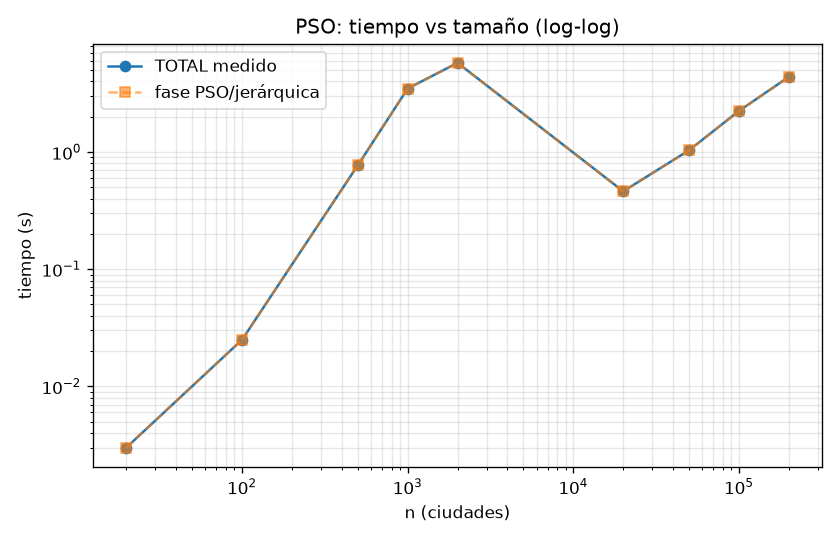
\includegraphics[width=.48\textwidth]{../docs/img_pso/fig_pso_tiempo.png}\hfill
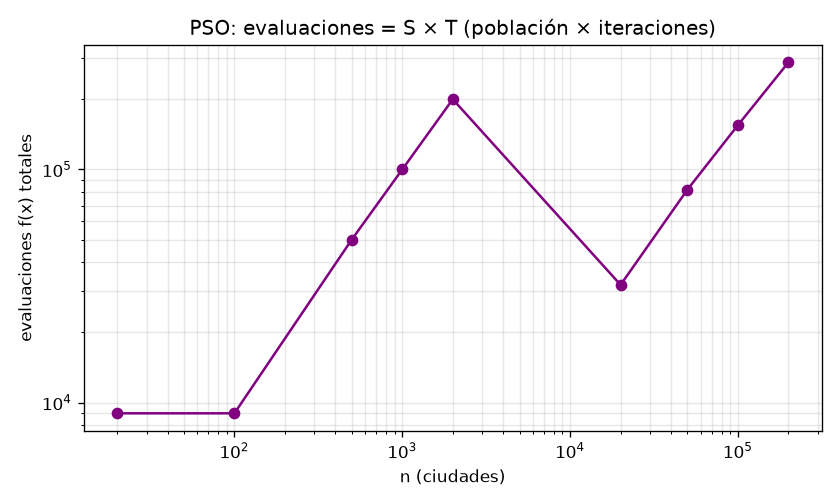
\includegraphics[width=.48\textwidth]{../docs/img_pso/fig_pso_evals.png}
\caption{Tiempo total vs $N$ (log-log) y evaluaciones $S\times T$. El tiempo cae en $N=20.000$ al entrar el régimen jerárquico (celdas de $\approx$900 con $S=32$ fijo): el costo lo dicta la arquitectura, no el enjambre. Nótese que el presupuesto de evaluaciones del régimen serie ($200.000$ en $N=2.000$) supera al jerárquico total ($288.000$ repartidas), pero produce un orden de magnitud menos calidad por evaluación.}
\end{figure}

\begin{figure}[H]\centering
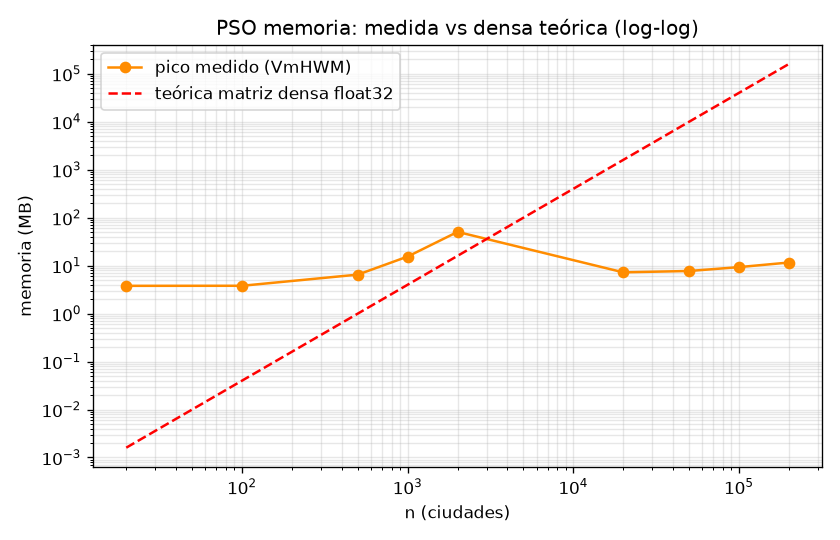
\includegraphics[width=.48\textwidth]{../docs/img_pso/fig_pso_memoria.png}\hfill
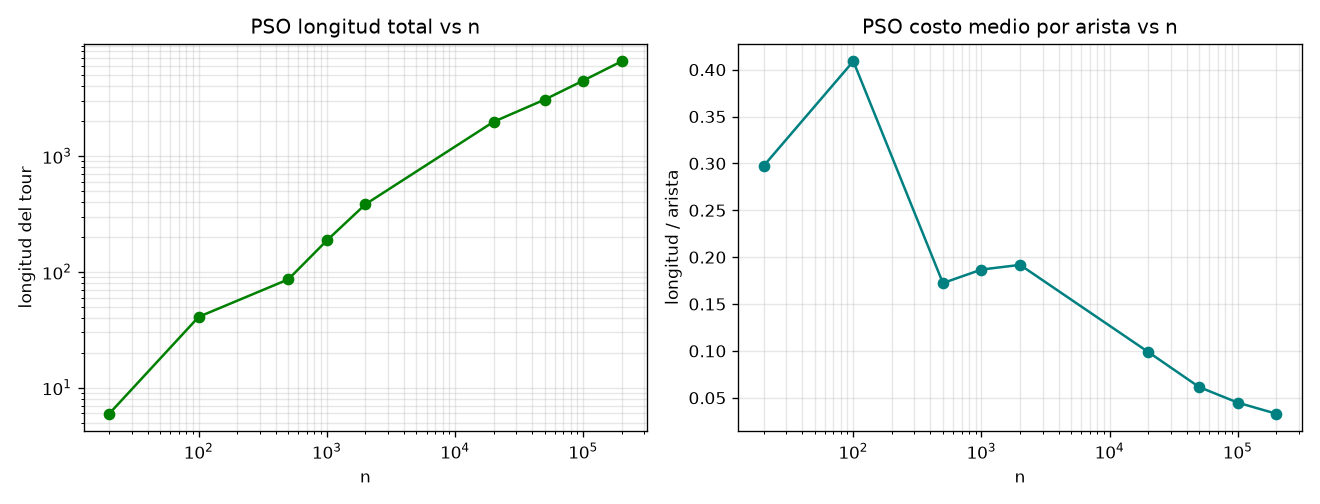
\includegraphics[width=.48\textwidth]{../docs/img_pso/fig_pso_calidad.png}
\caption{Memoria pico vs matriz densa teórica (izq.): $11{.}6\text{ MB}$ reales frente a $160\text{ GB}$ teóricos en 200k; la joroba en $N=2.000$ (50\,MB) es el enjambre $S\times N\times3$. Longitud y costo por arista $L/N$ (der.): $L/N$ se degrada un orden de magnitud con $N$, la firma de un tour sin estructura (cada arista cruza una fracción creciente del cuadrado).}
\end{figure}

\begin{figure}[H]\centering
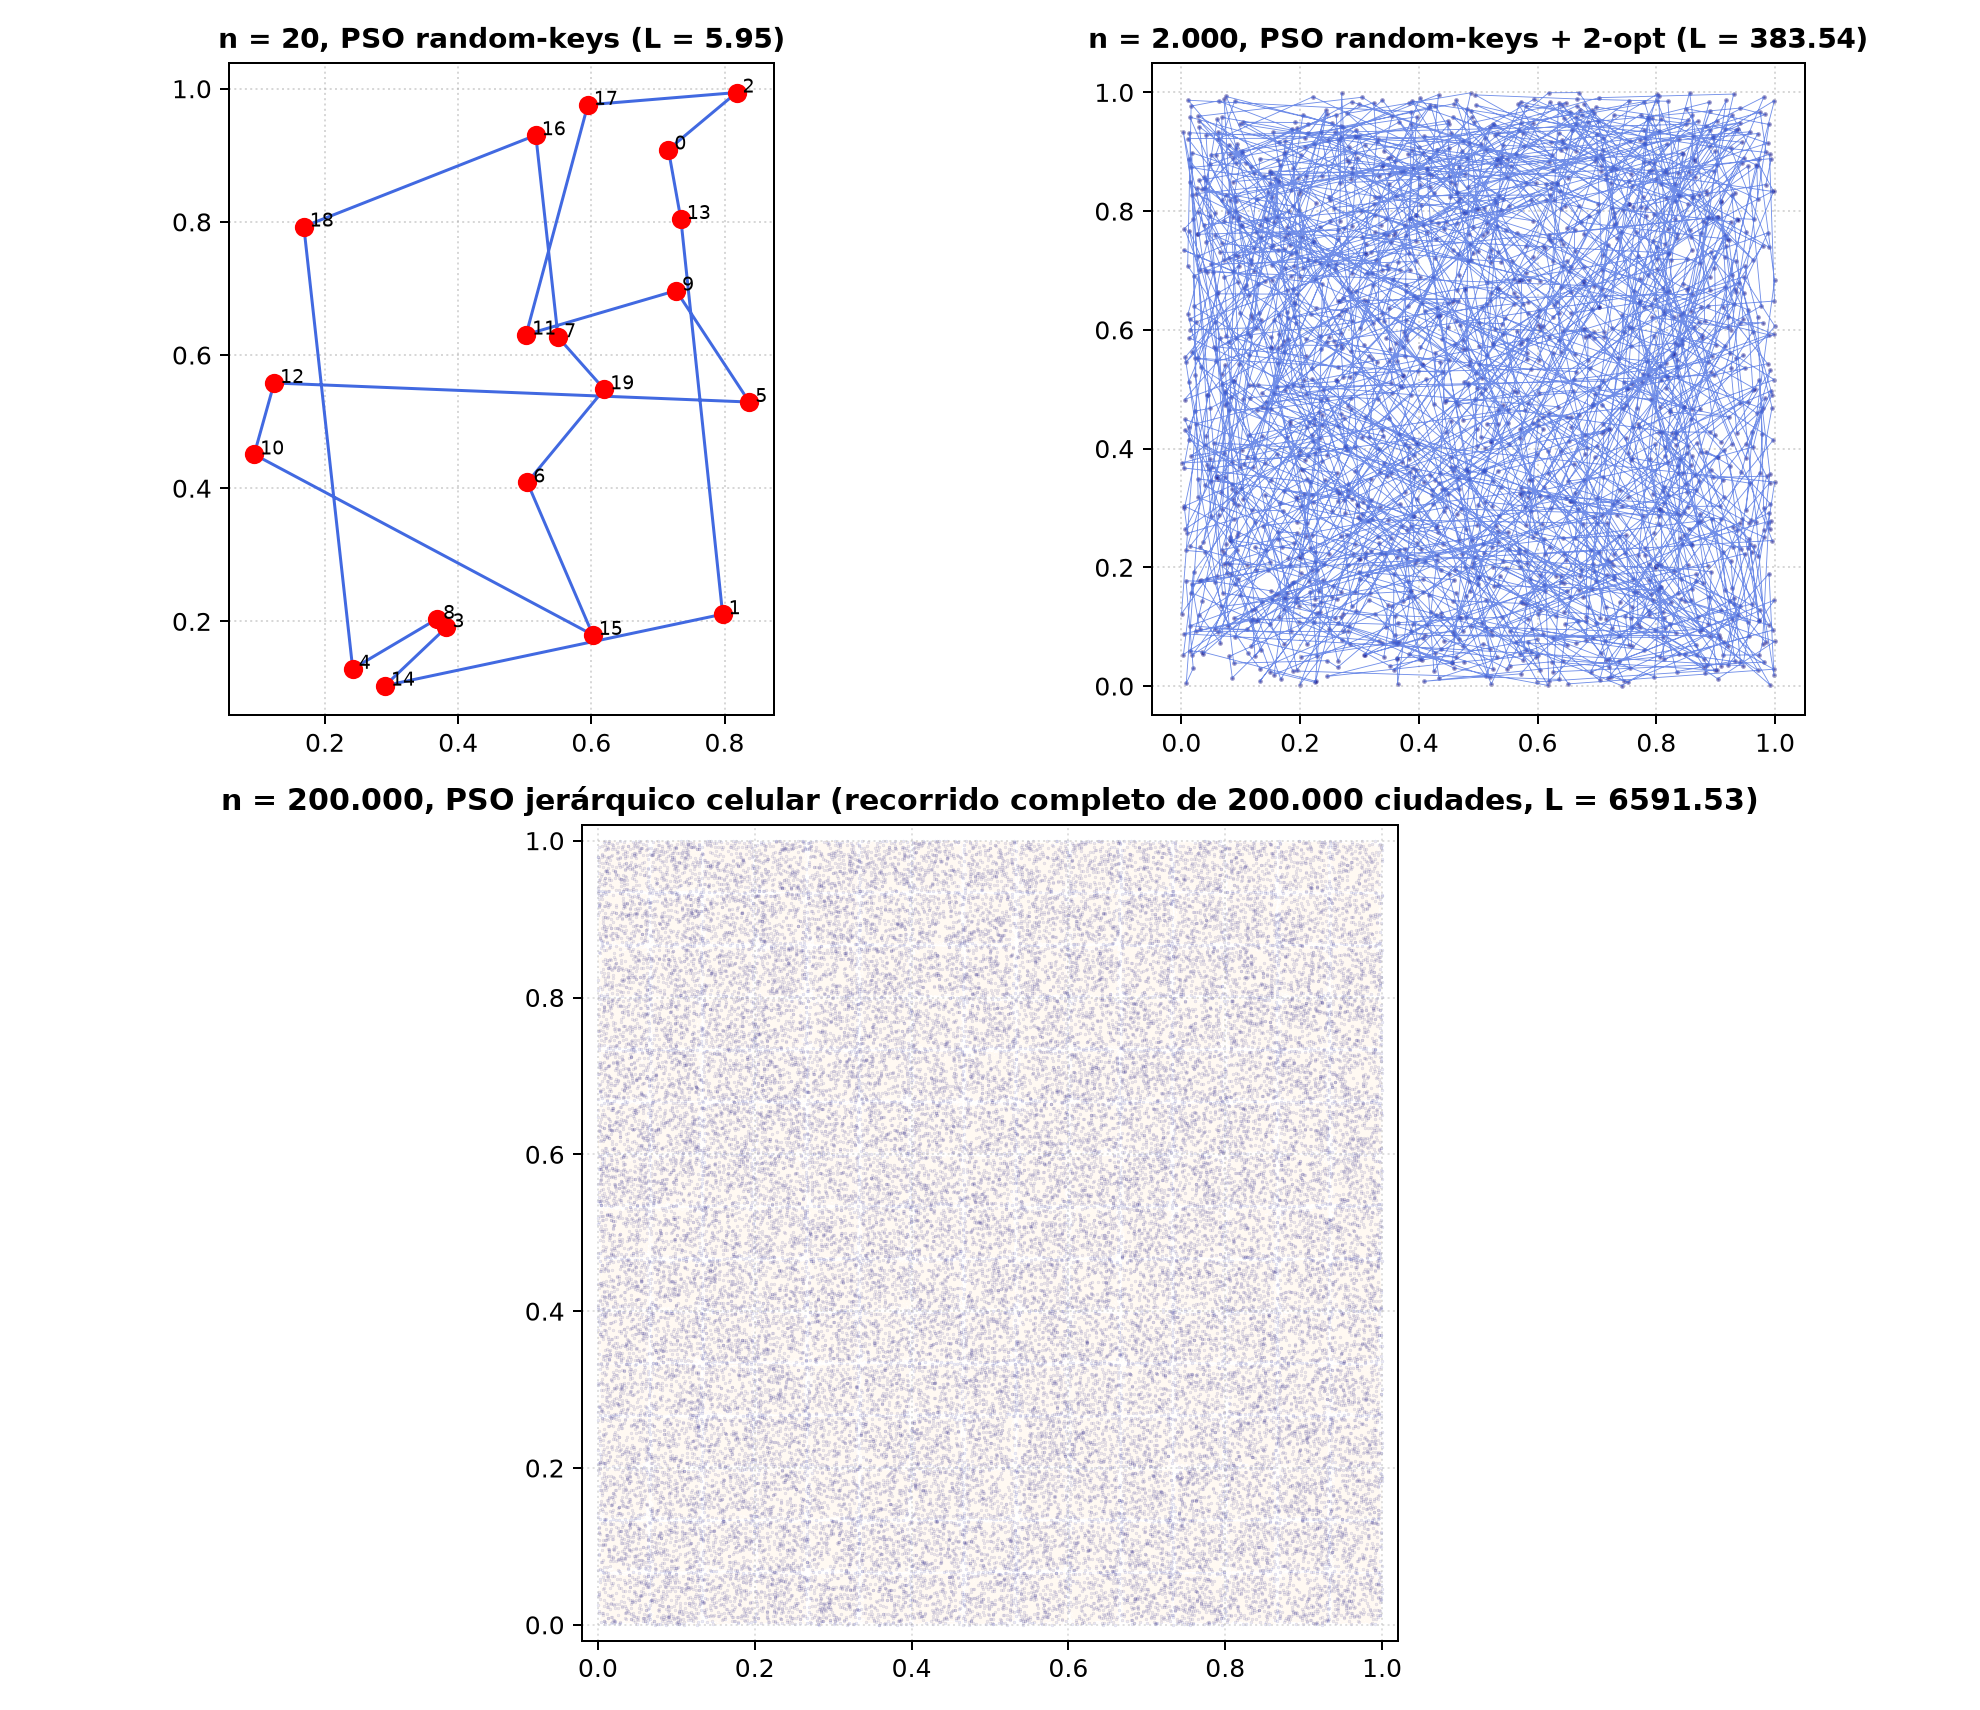
\includegraphics[width=\textwidth]{../docs/img_pso/fig_pso_tours.png}
\caption{Tours PSO (recorrido completo en los tres paneles). En $N=20$ se distinguen cruces evitables (p.ej.\ aristas que atraviesan todo el cuadrado); en $N=2.000$ domina la maraña de saltos largos; en $N=200.000$ cada celda es una madeja naranja y la cuadrícula $15\times15$ del esquema jerárquico queda al descubierto. Compárese con los tramos locales del ACO: mismo andamiaje, peor motor.}
\end{figure}

\subsection{Robustez Multi-Semilla y Estudio de Ablación}
\begin{center}
\begin{tabular}{@{}crr@{}}
\toprule $N$ (semillas) & longitud media $\pm$ std & mejor \\
\midrule 20 (5) & $5{.}70 \pm 0{.}52$ & 4.95 \\
2.000 (3) & $387{.}3 \pm 5{.}1$ & 381.52 \\
200.000 (2) & $6596{.}0 \pm 5{.}9$ & 6591.85 \\
\bottomrule
\end{tabular}
\end{center}
El método es estable ($\pm0.1$--$9\%$) alrededor de valores malos: la varianza entre réplicas es pequeña porque todas colapsan al mismo tipo de atractor. Ablación en $N{=}20$ (preguntas conceptuales de la guía): base 5.95, $c_1{=}0 \to 4{.}52$ (guía solo social: aquí ayuda), $c_2{=}0 \to 8{.}26$ (sin memoria colectiva, lo peor, como predice la teoría).

\begin{figure}[H]\centering
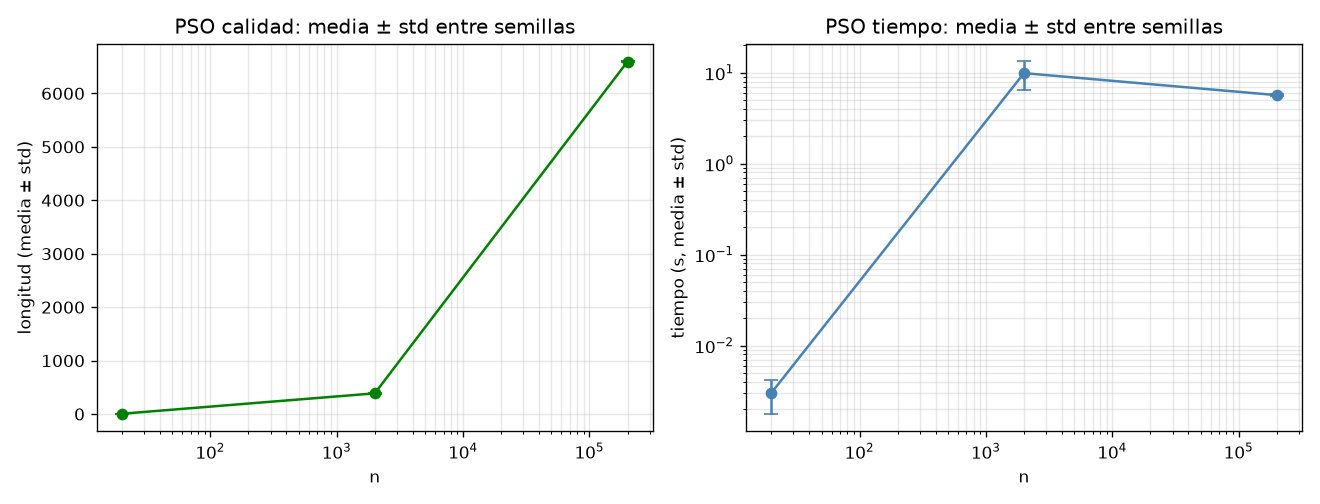
\includegraphics[width=.7\textwidth]{../docs/img_pso/fig_pso_semillas.png}
\caption{Media $\pm$ desviación entre semillas para longitud y tiempo. La calidad apenas se mueve con la semilla (el colapso es sistemático, no mala suerte); el tiempo en $N=2.000$ varía (7--12\,s) según cuándo dispara la parada temprana.}
\end{figure}

% ==============================================================================
\section{Discusión Técnica}
% ==============================================================================
¿Por qué el mismo andamiaje que lleva al ACO a +51\% deja al PSO en +1970\%? Tres causas encadenadas: (i) \textbf{representación sin localidad}: $argsort$ no preserva vecindad, así que el gradiente social apunta a ninguna parte útil; (ii) \textbf{arranque ciego}: el mejor de la inicialización en $N=2.000$ ($\approx$1010) ya está $30\times$ sobre el óptimo estimado y el enjambre nunca lo mejora (traza plana, parada en el primer instante); (iii) \textbf{colapso dimensional}: con $N$ dimensiones y $v_{\max}$ fijo, todas las partículas caen a la misma región de claves en pocas iteraciones (sensibilidad a $v_{\max}\in\{0{.}05,\dots,1{.}0\}$ probada: 4.59--5.95 en $N=20$, sin rescate). El 2-opt final rescata lo rescatable (1010 $\to$ 383) pero una pasada con ventana 40 no reconstruye un tour aleatorio. Conclusión didáctica: en combinatoria discreta, la codificación y el arranque aportan más que el motor de búsqueda.

% ==============================================================================
\section{Conclusiones}
% ==============================================================================
\begin{enumerate}
\item PSO fiel a las diapositivas (ecuaciones, $c_1{=}1{.}4$, $c_2{=}1{.}6$, $v_0=0$, $w$ decreciente, parada $S$) adaptado al TSP por claves aleatorias, en C++17 local, para $N=20$, $2.000$ y $200.000$ con medición de tiempo y memoria por fase.
\item La escala masiva es factible y barata ($4{.}5\text{ s}$, $11{.}6\text{ MB}$ vs $160\text{ GB}$ densos) gracias a la jerarquía celular, pero la calidad colapsa con $N$ (gap +87\% $\to$ +1970\%).
\item El método es estable entre semillas y responde a la ablación como predice la teoría ($c_2{=}0$ es lo peor), pero estable alrededor de un atractor malo.
\item Veredicto: para TSP discreto, un optimizador continuo con codificación ingenua no compite; su valor es demostrar cuantitativamente por qué la representación decide.
\end{enumerate}

\section*{Especificaciones de Validez y Límites Metodológicos}
Instancias uniformes en $[0,1]^2$ con el mismo generador y semillas que el ACO (tours directamente comparables). Presupuesto serie $S=N$ ($48\text{ MB}$ en $N=2.000$); celdas con $S=32$, $T=40$. Sin 2-opt en $N=20$; una pasada con ventana 40 en $N\in[200,5000]$. Tiempos medidos en CPU de 8 núcleos con OpenMP solo en el régimen jerárquico.

\section*{Referencias Bibliográficas}
\begin{itemize}
    \item Hurbans, R. (2020). \textit{Grokking Artificial Intelligence Algorithms}. Manning. Cap.~7.
    \item Kennedy, J., \& Eberhart, R. (1995). Particle swarm optimization. \textit{Proc.\ ICNN'95}, 1942--1948.
    \item Shi, Y., \& Eberhart, R. (1998). A modified particle swarm optimizer. \textit{IEEE ICEC}, 69--73.
    \item Reynolds, C. W. (1987). Flocks, herds and schools. \textit{Computer Graphics}, 21(4), 25--34.
\end{itemize}

\part{Comparativa ACO vs PSO}% =================================================================

\section{Protocolo comparativo}
Cinco prácticas estándar: (1) \textbf{mismas instancias} (generador idéntico; verificado por \texttt{diff}), (2) \textbf{mismo presupuesto} (población $\times$ iteraciones), (3) \textbf{multi-semilla} (3 corridas), (4) métrica \textbf{exceso\_\%} (media de cada algoritmo frente al mejor tour de \textit{cualquiera} de los dos) y (5) \textbf{trazas de convergencia}. Ningún binario fue modificado: \texttt{scripts/comparar\_aco\_pso.py} solo orquesta ambos binarios.
\begin{center}
\begin{tabular}{@{}clll@{}}
\toprule $N$ & ACO & PSO & presupuesto \\
\midrule 20 & \texttt{-a 20 -i 100} & \texttt{-S 20 -i 100} & $20\times100$ \\
2000 & \texttt{-a 20 -i 50} & \texttt{-S 20 -i 50} & $20\times50$ \\
200000 & \texttt{-a 8 -i 10} & \texttt{-S 8 -i 10} & $8\times10$ por celda \\
\bottomrule
\end{tabular}
\end{center}
En $N{=}20$ ningún algoritmo usa 2-opt (comparación pura del motor); en $N{=}2000$ ambos reciben el mismo pulido final con ventana 40.

\section{Resultados head-to-head}
\begin{center}
\begin{tabular}{@{}clrrrrr@{}}
\toprule $N$ & & media $\pm$ desv & mejor & tiempo & pico & exceso\_\% \\
\midrule 20 & ACO & $3{.}96 \pm 0{.}68$ & \textbf{3.19} & 0.003\,s & 3.9\,MB & 24.1 \\
   & PSO & $6{.}06 \pm 0{.}12$ & 5.94 & \textbf{0.001\,s} & 3.7\,MB & 90.1 \\
2000 & ACO & $\mathbf{41{.}53 \pm 0{.}07}$ & \textbf{41.46} & 0.32\,s & 4.2\,MB & 0.17 \\
   & PSO & $393{.}8 \pm 1{.}8$ & 391.75 & \textbf{0.10\,s} & 4.1\,MB & 849.9 \\
200k & ACO & $\mathbf{482{.}4 \pm 0{.}3}$ & \textbf{482.05} & 2.06\,s & 9.4\,MB & 0.08 \\
   & PSO & $6717 \pm 2$ & 6715.7 & \textbf{0.45\,s} & 8.9\,MB & 1293.5 \\
\bottomrule
\end{tabular}
\end{center}

\begin{figure}[H]\centering
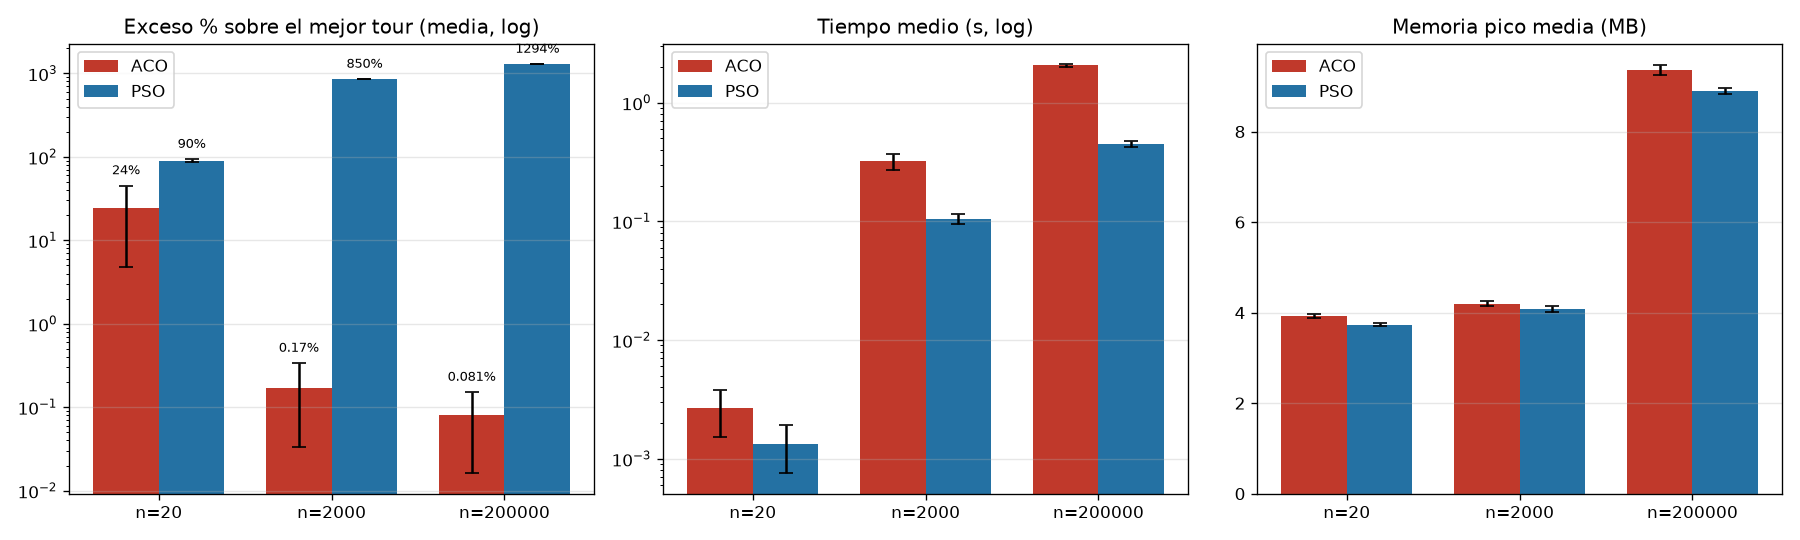
\includegraphics[width=\textwidth]{../docs/img_comp/fig_comp_barras.png}
\caption{Exceso sobre el mejor tour (izq.: dominancia en calidad, el ACO queda a $<1\%$ en 2000 y 200k), tiempo medio en log (centro: el PSO es $3$--$6\times$ más veloz; la escala logarítmica absorbe tres órdenes de magnitud) y memoria pico (der.: empate técnico, la dominan el binario y el pool OpenMP, no el algoritmo).}
\end{figure}

\begin{figure}[H]\centering
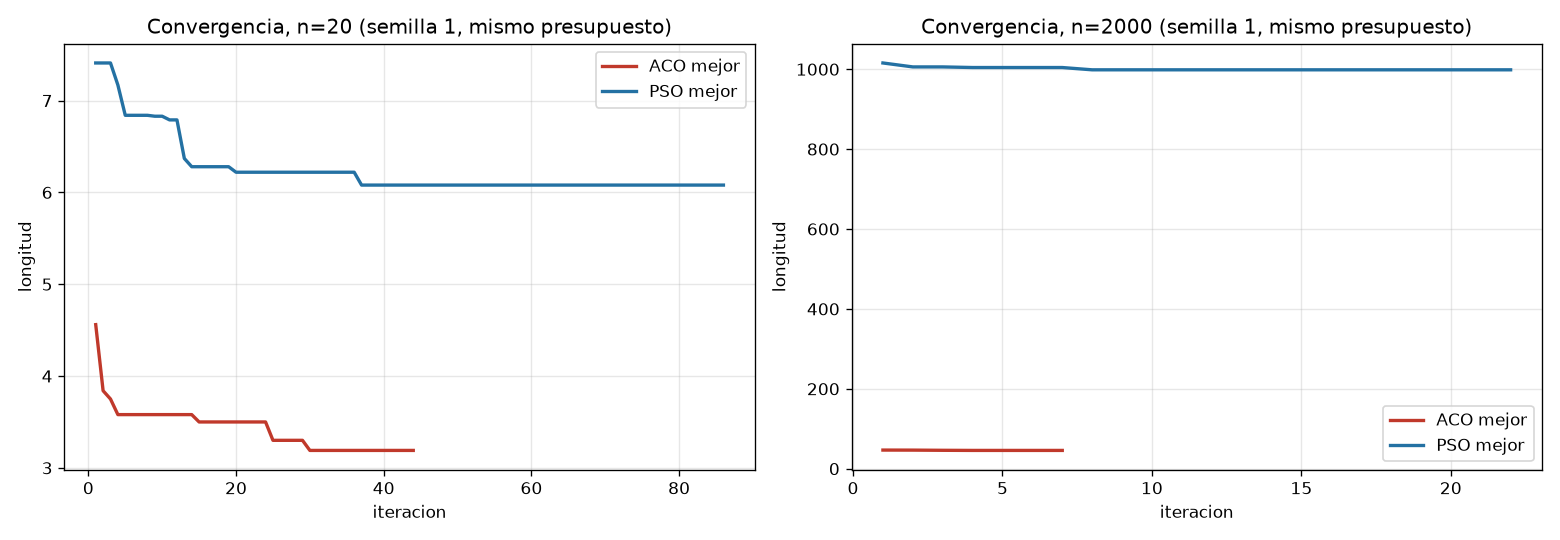
\includegraphics[width=\textwidth]{../docs/img_comp/fig_comp_convergencia.png}
\caption{Trazas del mejor global (semilla 1). En $N{=}20$ ambas descienden por escalones pero el ACO llega más lejos; en $N{=}2000$ el ACO nace bueno ($\approx$41, construcción heurística desde la iteración 1) y el PSO nace colapsado ($\approx$1000) y jamás mejora. La planitud no es optimalidad sino agotamiento de la diversidad.}
\end{figure}

\section{Discusión: lo que decide es el diseño, no la sigla}
La comparación pura en $N{=}20$ aísla el motor: el ACO (3.65) supera al PSO (5.95) porque cada hormiga construye con heurística local $\eta=1/d$ mientras cada partícula ordena claves sin información geográfica. En general, un PSO \textbf{discreto} (operadores sobre permutaciones, arranque NN, 2-opt por partícula) puede vencer a un ACO básico; simétricamente, el ACO aquí usado ($m{=}n$, doble feromona, elitismo) supera a un PSO continuo de arranque ciego. La moraleja es estable: representación, arranque y búsqueda local aportan más que la etiqueta del algoritmo.

\section{Conclusiones generales}
\begin{enumerate}
\item Con igualdad estricta, el \textbf{ACO vence en calidad en las tres escalas} a cambio de $2$--$5\times$ más tiempo; en memoria empatan ($<12\text{ MB}$).
\item El ahorro de recursos es arquitectónico y compartido: sin matrices densas, parada temprana y paralelismo por celdas, $200.000$ ciudades se resuelven en $<1$ minuto con $<12\text{ MB}$ donde el enfoque ingenuo exigiría $160\text{ GB}$.
\item El PSO continuo con codificación ingenua no compite en TSP discreto; su valor es didáctico y queda cuantificado en la Parte~I.
\end{enumerate}

\section*{Reproducibilidad general}
\begin{verbatim}
g++ -O3 -march=native -fopenmp -std=c++17 src/pso.cpp -o bin/pso
./bin/pso ; python3 scripts/barrido_pso.py ; python3 scripts/semillas_pso.py
python3 scripts/graficas_pso.py ; python3 scripts/comparar_aco_pso.py
\end{verbatim}
Entradas: \texttt{bin/aco}, \texttt{bin/pso} (sin modificar). Salidas: \texttt{data/pso\_*.csv}, \texttt{data/comp\_*.csv}, \texttt{docs/img\_pso/}, \texttt{docs/img\_comp/}, este PDF.
\end{document}
